\documentclass[conference]{IEEEtran}
\IEEEoverridecommandlockouts
% The preceding line is only needed to identify funding in the first footnote. If that is unneeded, please comment it out.
\usepackage{cite}
\usepackage{amsmath,amssymb,amsfonts}
\usepackage{amsmath, amsthm, amssymb}
\usepackage{algorithmic}
\usepackage{graphicx}
\usepackage{textcomp}
\usepackage{colortbl}
\usepackage{xcolor}
\usepackage{lipsum, babel}
\usepackage{listings}
\usepackage{color} %red, green, blue, yellow, cyan, magenta, black, white
\definecolor{mygreen}{RGB}{28,172,0} % color values Red, Green, Blue
\definecolor{mylilas}{RGB}{170,55,241}

\lstset{language=Matlab,%
    %basicstyle=\color{red},
    breaklines=true,%
    morekeywords={matlab2tikz},
    keywordstyle=\color{blue},%
    morekeywords=[2]{1}, keywordstyle=[2]{\color{black}},
    identifierstyle=\color{black},%
    stringstyle=\color{mylilas},
    commentstyle=\color{mygreen},%
    showstringspaces=false,%without this there will be a symbol in the places where there is a space
    numbers=left,%
    numberstyle={\tiny \color{black}},% size of the numbers
    numbersep=9pt, % this defines how far the numbers are from the text
    emph=[1]{for,end,break},emphstyle=[1]\color{red}, %some words to emphasise
    %emph=[2]{word1,word2}, emphstyle=[2]{style},    
}


\def\BibTeX{{\rm B\kern-.05em{\sc i\kern-.025em b}\kern-.08em
    T\kern-.1667em\lower.7ex\hbox{E}\kern-.125emX}}
\begin{document}

\title{Modelado y Control Backstepping de un Brazo Robótico de 6 GDL}

\author{\IEEEauthorblockN{Santiago Madariaga Collado}
\IEEEauthorblockA{\textit{Departamento de Ingeniería Electrónica} \\
\textit{Universidad de Ingeniería y Tecnología, Barranco 15063, Lima, Lima, Perú}\\
E-mail: santiago.madariaga@utec.edu.pe}
}

\maketitle
\begin{abstract}
En el presente informe se presenta el modelado y control backstepping de un brazo robotico de 6 grados de libertad no lineal de un robot de 6 grados de libertad. Para el modelado se utilizaron las ecuaciones de Lagrange para el modelado no lineal. En este paper se propone 1 controladores en este proyecto, un controlador backstepping. Para diseñar el sistema de control , empleando para ello la representactión en el espacio de estado del brazo robotico, así como también el algoritmo de control backstepping. Estos estudios de simulación demuestran que las 6 posiciones angulares del brazo robotico controladomsiguen simultáneamente a sus señalesde referencia para el caso de regulación (referencias constantes), y para el caso de seguimiento (señales cambiantes arbritrarias). Cumoliendo los parámetros preestablecidos. 
\end{abstract} 

\begin{IEEEkeywords}
modelado dinámico brazo robótico, control backstepping, simulación no lineal, método de Euler-Lagrange.
\end{IEEEkeywords}

% igual que el resumen pero mas extenso
% indicar que este trabajo es una extension de trabajos previos de menos DOF. Explicar el método de Euler y su uso en este caso. Buscar trabajos similares y aplicación de los brazos de 6 dof.
\section{Introducción}
En el presente trabajo, el modelo dinámico MIMO de un robot de 6 GDL es obtenido usando el método de las ecuaciones de Lagrange. Para el control del brazo robótico, se diseñó un controlador con el método de Backstepping. Este controlador esta basado en el modelo del brazo debido a que el diseño de este controlador requiere el modelo dinámico del brazo robotico.\\
El objectivo del sismta de control es diseñar un vector de contrul $u$ que haga a las 6 salidas del controlador seguir las trayectorias mostradas, en el modo de seguimiento, y alcanzar el valor de referencia cuando las señales de referencia son constantes.  Se utilizó el código de un controlador backstepping diseñado para un brazo robot de 3 GDL como punto de partida[1]. Además, el modelo del sistema parte de trabajos previos de brazos de 3 GDL[2]. Se utilizó el modo simbólico de MATLAB para hallar los valores de las matrices y realizar la simulación del controlador backstepping. 


\section{Modelado del Brazo Robótico de 6GDL}
La dinámica del robot se ocupa de la relación entre las fuerzas que actúan
sobre un cuerpo y el movimiento que en él se origina. Por tanto, el modelo dinámico de un robot tiene por objetivo conocer la relación entre el movimiento del robot y las fuerzas implicadas en el mismo.\\
Esta relación se obtiene mediante el denominado modelo dinámico, que establece la relación matemática entre las entradas (señal de control) y las salidas (ángulos).


\begin{figure} [h]
\centering
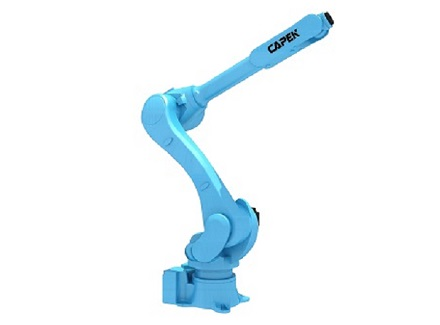
\includegraphics[width=0.53\textwidth]{images/6dof_arm.jpg}
\caption{Robot industrial de 6GDL[3]}
\end{figure}

El modelo extraído de [1] consiste de un brazo robótico de 3GDL, este modelo se expandió para el modelado de un brazo robótico de 6GDL. El modelo del brazo robótico es expresado como:
\begin{equation}
M(q)\dot + P(q,\dot{q})\dot{q} + d(q) = u
\end{equation}
Donde $M(q)\ddot{q}$ es la matriz de inercia, es simétrica 6x6. El término $P(q, \dot{q})\dot{q}$ incluye las fuerzas centrípetas y de Coriolis. Por último, el vector 'd' contiene la gravedad y demás términos que actuan en las uniones del brazo robótico. \\
Para obtener al modelo en la forma matricial (1) se debe de unir la parte mecánica y eléctrica. Es decir, las ecuaciones dinámicas que describen a los ángulos (que son las salidas del sistema a controlar) en términos del modelo mecánico del sistema (velocidad y energía potencial), deben relacionarse con las entradas del sistema, las cuales son los voltajes. Esto se logra utilizando las ecuaciones de lagrange, las cuales relacionan torques y energías.

\begin{equation}
L = V - U
t_i = \frac{d}{dt}\frac{\partial L }{\partial \dot{q_i}} - \frac{\partial L}{\partial q_i}\\
\end{equation}

Donde $V$ y $P$ son la sumatoria de energías cinéticas y potenciales respectivamente.



Los valores de los parámetros se tomaron de [2]. A continuación se muestra la tabla extraída de la misma referencia.


\onecolumn

Para hallar la relación entre torques y voltajes, se debe de realizar el análisis eléctrico del motor.
\begin{figure} [h]
    \centering
    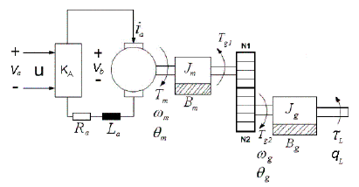
\includegraphics[width=0.3\textwidth]{images/engine.png}
    \caption{Diagrama del actuador del brazo robótico}
\end{figure}

Ecuaciones del actuador:
$$\tau_i = -J_{eq}\ddot{q_i} - (B_{eq} + \frac{n^2K_m K_b}{R_a})*\dot{q_i} + \frac{n K_m K_A}{R_a} u_i$$\\

\begin{table}
\centering
\begin{tabular}{|l|l|l|l|} 
\hline
\rowcolor[rgb]{0.725,0.729,0.733} Símbolo & Descripcióon                                       & Valor     & Unidades   \\ 
\hline
u1, u2, u3                                & Voltaje de entrada a cada actuador                 &        & V          \\ 
\hline
u                                         & Voltaje de entrada a un actuador                   &        & V          \\ 
\hline
KA                                        & Ganancia del amplificador                          & 8.5       &        \\ 
\hline
Va                                        & Voltaje de armadura                                &        & V          \\ 
\hline
Ra                                        & Resistencia de armadura                            & 2.49      & Ω          \\ 
\hline
La                                        & Inductancia de armadura                            & 2.63×10−3 & H          \\ 
\hline
ia                                        & Corriente de armadura                              & A         &         \\ 
\hline
Km                                        & Constante del torque motor                         & 0.0458    & N-m/A      \\ 
\hline
Tm                                        & Torque motor                                       &        & N-m        \\ 
\hline
τL                                        & Torque de carga                                    &        & N-m        \\ 
\hline
Tg1                                       & Torque de entrada a los engranajes                 &        & N-m        \\ 
\hline
Tg2                                       & Torque de salida de los engranajes                 &        & N-m        \\ 
\hline
Jm                                        & Inercia del motor                                  & 7.1×10−6  & kg-m2      \\ 
\hline
Jg                                        & Inercia de los engranajes                          & 0.053     & kg-m2      \\ 
\hline
Ja                                        & Inercia del eje o arbol conectado al motoresductor &        & kg-m2      \\ 
\hline
Jr                                        & Inercia del rodamiento conectado al arbol          &        & kg-m2      \\ 
\hline
J1                                        & Inercia de la columna                              &        & kg-m2      \\ 
\hline
J2                                        & Inercia del brazo                                  &        & kg-m2      \\ 
\hline
J3                                        & Inercia del antebrazo                              &        & kg-m2      \\ 
\hline
Bm                                        & Constante de friccion del motor                    & 0.0001    & N-m/rad/s  \\ 
\hline
Bg                                        & Constante de friccion en engranajes                & 0.01      & N-m/rad/s  \\ 
\hline
ma                                        & Masa del eje o arbol conectado al motoreductor     & 1.5       & kg         \\ 
\hline
mr                                        & Masa del rodamiento conectado al arbol             & 1.48      & kg         \\ 
\hline
m1                                        & Masa total de la columna                           & 2.98      & kg         \\ 
\hline
m2                                        & Masa del brazo                                     & 0.89      & kg         \\ 
\hline
m3                                        & Masa del antebrazo                                 & 0.25      & kg         \\ 
\hline
la                                        & Longitud del eje o arbol conectado al motoreductor & 0.3378    & m          \\ 
\hline
lr                                        & Longitud del rodamiento y disco conectado al arbol & 0.054     & m          \\ 
\hline
L1                                        & Longitud total de la columna                       & 0.391     & m          \\ 
\hline
L2                                        & Longitud del brazo                                 & 0.24      & m          \\ 
\hline
L3                                        & Longitud del antebrazo                             & 0.245     & m          \\ 
\hline
ra                                        & Radio del eje o arbol conectado al motoreductor    & 0.015     & m          \\ 
\hline
rr                                        & Radio del rodamiento y disco conectado al arbol    & 0.0427    & m          \\ 
\hline
Vb                                        & Voltaje contraelectromotriz                        &        & V          \\ 
\hline
Kb                                        & Constante contraelectromotriz                      & 0.0458    & V/rad/s    \\ 
\hline
g                                         & Aceleracion de la gravedad                         & 9.81      & m/s2       \\ 
\hline
N1, N2~                                   & No de dientes de los engranajes (N2  N1)           &        &         \\ 
\hline
n                                         & Relacion de engranajes (n = N2/N1)                 & 65.5      &         \\ 
\hline
θm                                        & Posicion angular del motor                         &        & rad        \\ 
\hline
θg                                        & Posicion angular del eje de salida del motor       &        & rad        \\ 
\hline
ωm                                        & Velocidad angular del motor (ωm = nωg)             & rad/s     &         \\ 
\hline
ωg                                        & Velocidad angular de la carga                      &        & rad/s      \\ 
\hline
qL                                        & Coordenada articular de un eslabon                 &        & rad        \\ 
\hline
q1, q2, q3                                & Coordenadas articulares para cada eslabon          &        & rad        \\
\hline
\end{tabular}\\
Tabla 1: Parámetros y variables del brazo robótico de 6GDL
\end{table}
\newpage
\twocolumn

\subsection{Modelado del Sistema en MATLAB}
El modelado del sistema se llevó a cabo definiendo los parámetros y las variables del sistema en el modo simbólico de MATLAB, permitiendo inspeccionar las relaciones entre las variables del sistema. El modo simbólico también permite hallar las derivadas parciales y totales, las cuales son necesarias para hallar las ecuaciones de Lagrange.\\
Código de matlab: q1\_d(t) = diff(q1(t))\\
Salida: $$\frac{\partial }{\partial t}\;q_2 \left(t\right)$$
Esto se realizará con todos los ángulos.
En segundo lugar, se definen las coordenadas en el espacio de cada unión del brazo robótico:

\lstinputlisting{coordenadas.m}
Como se Puede observar en el código, las coordenadas mayores dependen de las anteriores. Al momento de expandir las expresiones en función de los parámetros y no las variables, las expresiones resultantes tienen un tamaño considerable. Sin embargo, al reemplazar los parámetros por valores numéricos las expresiones se reducen. \\
Posteriormente, se hallan las energías (potencial y cinética) de los segmentos del brazo. 
\begin{lstlisting}
% Energias: 
syms J1 J2 J3 J4 J5 J6
V1 = 1/2*J1*q1_d(t)^2;
U1 = m1*g*(ma*la + mr*lr)/(ma + mr);

V2 = 1/2*J2*q2_d(t)^2 + 1/2*m2*(x2_d^2 + y2_d^2 + z2_d^2);
U2 = m2*g*(L1 + L2/2*cos(q2(t)));

V3 = 1/2*J3*q3_d(t)^2 + 1/2*m3*(x3_d^2 + y3_d^2 + z3_d^2);
U3 = m3*g*z3;

V4 = 1/2*J4*q4_d(t)^2 + 1/2*m4*(x4_d^2 + y4_d^2 + z4_d^2);
U4 = m4*g*z4;

V5 = 1/2*J5*q5_d(t)^2 + 1/2*m5*(x5_d^2 + y5_d^2 + z5_d^2);
U5 = m5*g*z5;

V6 = 1/2*J6*q6_d(t)^2 + 1/2*m6*(x6_d^2 + y6_d^2 + z6_d^2);
U6 = m6*g*z6;
\end{lstlisting}
Con las expresiones de las energías conocidas, se aplica las ecuaciones de Lagrange para hallar los torques.
\begin{lstlisting}
V = V1 + V2 + V3 + V4 + V5 + V6;
U = U1 + U2 + U3 + U4 + U5 + U6;
L = simplify(expand(V - U));
\end{lstlisting}
Posteriormente, se calculan los torques para cada ángulo de la siguiente forma:\\

$$t_i = \frac{d}{dt}\frac{\partial L }{\partial \dot{q_i}} - \frac{\partial L}{\partial q_i}$$\\

Esto se aplicará para todos los ángulos, $i \in [1,6]$.\\
Luego se hallan las dobles derivadas de los ángulos y se relacionan las entradas y los torques con la siguiente ecuación:
$$\tau_i = -J_{eq}\ddot{q_i} - (B_{eq} + \frac{n^2K_m K_b}{R_a})*\dot{q_i} + \frac{n K_m K_A}{R_a} u_i$$\\
\newpage
\onecolumn
Esto empleado para todas las salidas del sistema: $i \in [1,6]$.\\
Por último, despejando las entradas (voltajes) $u$ de las 6 ecuaciones y la expresión en MATLAB es la siguiente
\begin{lstlisting}
u1 = (t1 - (-Jeq*q1dd - (Beq + n^2*Km*Kb/Ra)*q1_d(t)))*Ra/(n*Km*Ka);
u2 = (t2 - (-Jeq*q2dd - (Beq + n^2*Km*Kb/Ra)*q2_d(t)))*Ra/(n*Km*Ka);
u3 = (t3 - (-Jeq*q3dd - (Beq + n^2*Km*Kb/Ra)*q3_d(t)))*Ra/(n*Km*Ka);
u4 = (t4 - (-Jeq*q4dd - (Beq + n^2*Km*Kb/Ra)*q4_d(t)))*Ra/(n*Km*Ka);
u5 = (t5 - (-Jeq*q5dd - (Beq + n^2*Km*Kb/Ra)*q5_d(t)))*Ra/(n*Km*Ka);
u6 = (t6 - (-Jeq*q6dd - (Beq + n^2*Km*Kb/Ra)*q6_d(t)))*Ra/(n*Km*Ka);
\end{lstlisting}
Donde qidd es la doble derivada del ángulo número $i$.\\
\\

Con las expresiones de las entradas se arman las matrices del modelo dinámico del sistema, de la siguiente forma.
\begin{equation}
    u_1 = M_{11}\ddot{q_1} + P_{11}\dot{q_1} + P_{12}\dot{q_2 + P_{13}\dot{q_3}} + P_{14}\dot{q_4} + P_{15}\dot{q_5} + P_{16}\dot{q_6}
\end{equation}

\begin{equation}
    u_2 = M_{22}\ddot{q_2} + M_{23}\ddot{q_3} + M_{24}\ddot{q_4} + M_{25}\ddot{q_5} + M_{26}\ddot{q_6}+ P_{21}\dot{q_1} + P_{12}\dot{q_2d + P_{13}\dot{q_3}} + P_{14}\dot{q_4} + P_{15}\dot{q_5} + P_{16}\dot{q_6} + d_{2}
\end{equation}

\begin{equation}
    u_3 = M_{32}\ddot{q_3} + M_{33}\ddot{q_3} + M_{34}\ddot{q_4} + M_{35}\ddot{q_5} + M_{36}\ddot{q_6}+ P_{31}\dot{q_1} + P_{32}\dot{q_2d + P_{33}\dot{q_3}} + P_{34}\dot{q_4} + P_{35}\dot{q_5} + P_{36}\dot{q_6} +
    d_{3}    
\end{equation}

\begin{equation}
    u_4 = M_{42}\ddot{q_2} + M_{43}\ddot{q_3} + M_{44}\ddot{q_4} + M_{45}\ddot{q_5} + M_{46}\ddot{q_6}+ P_{41}\dot{q_1} + P_{42}\dot{q_2d + P_{43}\dot{q_3}} + P_{44}\dot{q_4} + P_{45}\dot{q_5} + P_{46}\dot{q_6} +
    d_{4}
\end{equation}

\begin{equation}
    u_5 = M_{52}\ddot{q_2} + M_{53}\ddot{q_3} + M_{54}\ddot{q_4} + M_{55}\ddot{q_5} + M_{56}\ddot{q_6}+ P_{51}\dot{q_1} + P_{52}\dot{q_2d + P_{53}\dot{q_3}} + P_{54}\dot{q_4} + P_{55}\dot{q_5} + P_{56}\dot{q_6} +
    d_{5}
\end{equation}

\begin{equation}
    u_6 = M_{62}\ddot{q_2} + M_{63}\ddot{q_3} + M_{64}\ddot{q_4} + M_{65}\ddot{q_5} + M_{66}\ddot{q_6}+ P_{61}\dot{q_1} + P_{62}\dot{q_2d + P_{63}\dot{q_3}} + P_{64}\dot{q_4} + P_{65}\dot{q_5} + P_{66}\dot{q_6} +
    d_{6}
\end{equation}

\\
Dado que se conocen las ecuaciones de las entradas, para hallar cada valor de las matrices se debe de factorizar los coeficientes de las variables de control respectivas. Este proceso se llevó a cabo con las funciones $coeffs()$ y $collect()$ en MATLAB. 
Luego, se arman las matrices con el siguiente código:
\begin{lstlisting}
% Matriz M:
M = [M11 0 0 0 0 0;
    0 M22 M23 M24 M25 M26;
    0 M32 M33 M34 M35 M36;
    0 M42 M43 M44 M45 M46;
    0 M52 M53 M54 M55 M56;
    0 M62 M63 M64 M65 M66;];


% Patriz P:
P = [P11 P12 P13 P14 P15 P16;
    P21 P22 P23 P24 P25 P26;
    P22 P32 P33 P34 P35 P36;
    P23 P42 P43 P44 P45 P46;
    P24 P52 P53 P54 P55 P56;
    P25 P62 P63 P64 P65 P66;];

% Vector D:
D = [0; d21; d31; d41; d51; d61];
\end{lstlisting}
Con las matrices M y P, además del vector D, el modelo dinámico del sistema está completo y listo para probar el controlador seleccionado, en este caso el controlador backstepping.

\newpage
\twocolumn
\section{El Algoritmo Backstepping}
El controlador backstepping fue diseñado usando el código de [1] como punto de partida. El algoritmo en cuestión tiene la siguiente forma:
\begin{equation}
    u = M(q)\ddot{q_d} + P(q,\dot{q})\dot{q_r} + d(q) - K_d(\dot{q} - \dot{q_r}) - K_1 z_1
\end{equation}
$K_d$ y $K_1$ son matrices diagonales con elementos positivos. El error de seguimiento $z$ se define de la siguiente forma:
\begin{equation}
    z_1 = q - q_d
\end{equation}

Donde $q$ es el vector de posiciones medidas y $q_d$ es el vector de las trayectorias deseadas. \\
La estimación del vector $\dot{q}$ del vector conocido $q$ es la siguiente:
\begin{equation}
    \dot{\hat{q}} = \dot{q_d} + L_d(q - \hat{q})
\end{equation}
$L_d$ es uan matriz diagonal con elementos positivos.\\
El controlador backstepping resultante es el siguiente:
\begin{equation}
    u = M(q)\ddot{q_d} + P(q,\dot{\hat{q}})\dot{q_r} + d(q) - K_d(\dot{\hat{q}} - \dot{q_r}) - K_1 z_1
\end{equation}

\section{Simulación en MATLAB}
Para llevar a cabo la simulación, se sustituyeron las constantes simbólicas por el valor del parámetro que representaban. Esto se llevó a cabo utilizando la función $subs()$.\\
Sin embargo, debido a que las salidas (los ángulos) aún están presentes en las matrices, las matrices se deben de convertir a un objecto en MATLAB que permita la rápida sustitución de sus valores para la simulación. El modo simbólico no es apto para este caso ya que éste representa las operaciones de números racionales en forma fraccionaria y no decimal. Dicho cálculo tarda un tiempo considerable. Por lo tanto, las matrices simbólicas se convirtieron en funciones one-line de MATLAB, usando el siguiente código:

\begin{lstlisting}
M = matlabFunction(vpa(simplify(expand(M))));
P = matlabFunction(vpa(simplify(expand(P))));
D = matlabFunction(vpa(simplify(expand(D))));
\end{lstlisting}

En primer lugar, se expande la expresión simbólica de cada matriz para poder reagrupar los coeficientes de las variables, en segundo lugar, se simplifica la expresión expandida y se utiliza la función vpa() para convertir las fracciones simbólicas en expresiones de punto flotante, sin embargo, los ángulos aún son expresiones simbólicas. Por último, la función matlabFunction() convierte a la expresión simbólica resultante en una función de matlab la cual tiene los ángulos como parámetros. La función resultante tiene la siguiente forma:

\begin{lstlisting}
M = function_handle with value: 
@(q2_,q3_,q4_,q5_,q6_)reshape([sin(q2_).*sin(q3_). [...]
\end{lstlisting}

Al tener las matrices en forma de funciones se puede proceder a simular el controlador en MATLAB. Se definen los parámetros del controlador, los valores iniciales, el tiempo de muestreo y las referencias deseadas.


\section{Resultados de la simulación}
La simulación de seguimiento se llevó a cabo con un tiempo de 10 segundos, mientras que en la simulación con referencias constantes el tiempo fue de 4 
segundos.

\subsection{Simulación con referencias constantes}

\begin{figure} [h]
\centering
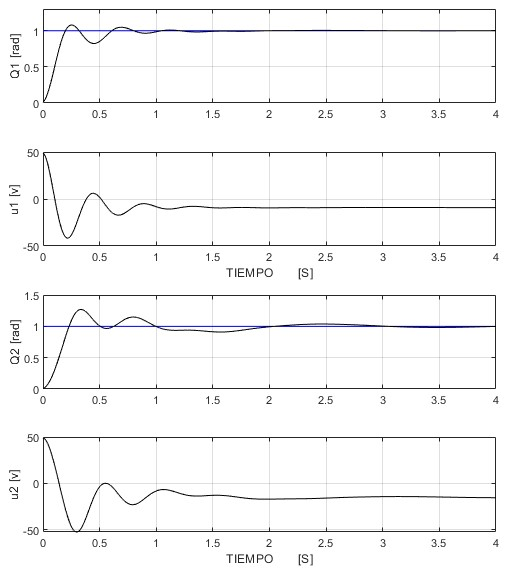
\includegraphics[width=0.4\textwidth]{images/normal/q1_q2.jpg}
\caption{Señales de entrada y salida 1 y 2}
\end{figure}


\begin{figure} [h]
\centering
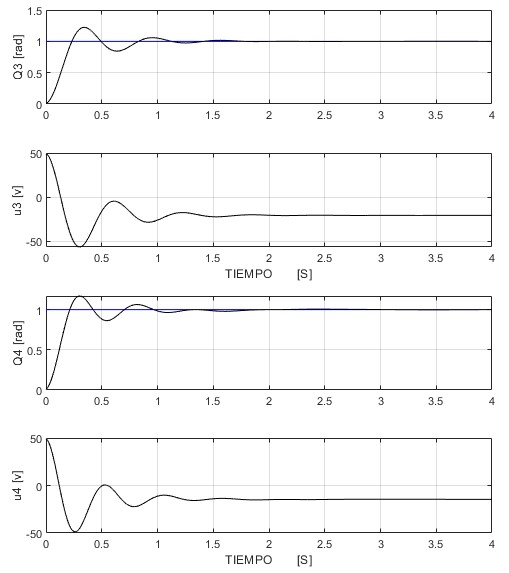
\includegraphics[width=0.4\textwidth]{images/normal/q3_q4.jpg}
\caption{Señales de entrada y salida 3 y 4}
\end{figure}


\begin{figure} [h]
\centering
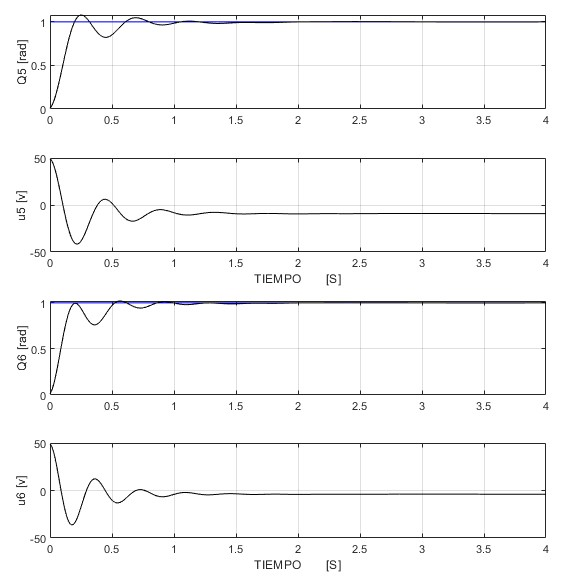
\includegraphics[width=0.4\textwidth]{images/normal/q5_q6.jpg}
\caption{Señales de entrada y salida 5 y 6}
\end{figure}



\subsection{Simulación de seguimiento}
\begin{figure} [h]
\centering
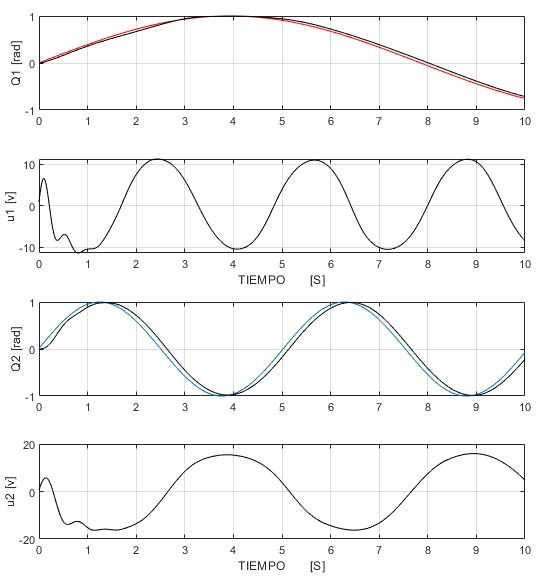
\includegraphics[width=0.4\textwidth]{images/seguimiento/q1_q2_seg.jpg}
\caption{Señales de entrada y salida 1 y 2}
\end{figure}


\begin{figure} [h]
\centering
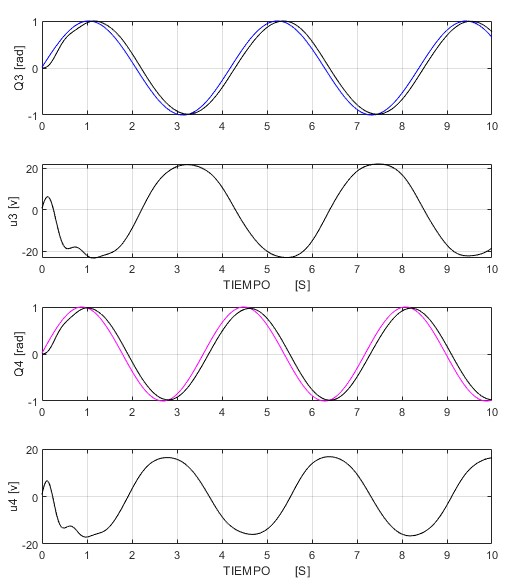
\includegraphics[width=0.4\textwidth]{images/seguimiento/q3_q4_seg.jpg}
\caption{Señales de entrada y salida 3 y 4}
\end{figure}


\begin{figure} [h]
\centering
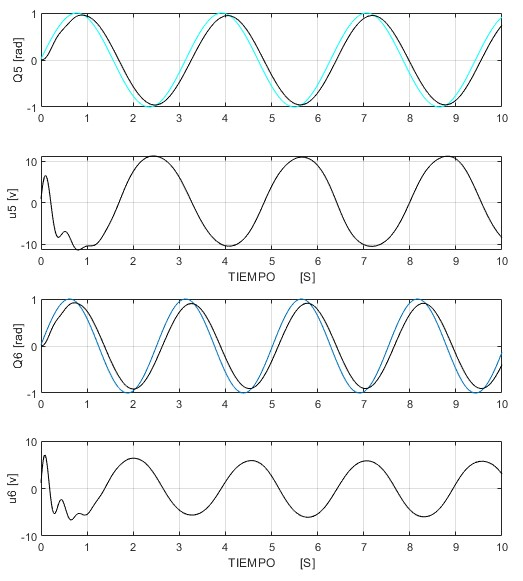
\includegraphics[width=0.4\textwidth]{images/seguimiento/q5_q6_seg.jpg}
\caption{Señales de entrada y salida 5 y 6}
\end{figure}


\newpage
\section{Conclusiones}
El modelado del sistema se llevó a cabo de manera eficiente utilizando el modo simbólico de MATLAB. El algoritmo backstepping es del tipo que se basa en el modelo ya que requiere el modelo dinámico del brazo robótico.  \\
El modo simbólico en MATLAB no es eficiente para su uso en el lazo de control, por lo tanto las variables simbólicas deben convertirse en una función de MATLAB para simular el controlador.\\
Todas las salidas del sistema de control diseñado fueron capaces de seguir las señales arbitrarias diseñadas deseadas, cumpliendo los parámetros establecidos: un overshoot menor al 10\%. un tiempo de establecimiento menor a 3 segundos y un error en estado estable menor al 1\%.

\begin{thebibliography}{00}
\bibitem{b1} H. Ventura, "Diseño e Imlementación de un Controlador Fuzzy Adaptativo para un Brazo Robótico de 3GL", Editorial: UNI, 2017
\bibitem{b2} A. Rojas, “Control No Lineal Multivariable”, Editorial: UNI, 2012
\bibitem{b3} ROBOT INDUSTRIAL DE 6 GRADOS DE LIBERTAD  (s.f.) [fotografía] http://equinlabsac.com/sites/default/files/5b74439912482.jpg
\end{thebibliography}
\vspace{12pt}
\end{document}
